\documentclass[aspectratio=169]{beamer}

\mode<presentation>
{
  \usetheme{default}
  \usecolortheme{default}
  \usefonttheme{default}
  \setbeamertemplate{navigation symbols}{}
  \setbeamertemplate{caption}[numbered]
  \setbeamertemplate{footline}[frame number]  % or "page number"
  \setbeamercolor{frametitle}{fg=white}
  \setbeamercolor{footline}{fg=black}
} 

\usepackage[english]{babel}
\usepackage[utf8x]{inputenc}
\usepackage{tikz}
\usepackage{courier}
\usepackage{array}
\usepackage{bold-extra}
\usepackage{minted}
\usepackage[thicklines]{cancel}

\xdefinecolor{dianablue}{rgb}{0.18,0.24,0.31}
\xdefinecolor{darkblue}{rgb}{0.1,0.1,0.7}
\xdefinecolor{darkgreen}{rgb}{0,0.5,0}
\xdefinecolor{darkgrey}{rgb}{0.35,0.35,0.35}
\xdefinecolor{darkorange}{rgb}{0.8,0.5,0}
\xdefinecolor{darkred}{rgb}{0.7,0,0}
\definecolor{darkgreen}{rgb}{0,0.6,0}
\definecolor{mauve}{rgb}{0.58,0,0.82}

\title[2018-07-07-pyhep-pythonhistory]{The Python Scientific Software Ecosystem: \\ Past, Present and Future}
\author{Jim Pivarski}
\institute{Princeton University -- DIANA-HEP}
\date{July 7, 2018}

\begin{document}

\logo{\pgfputat{\pgfxy(0.11, 7.4)}{\pgfbox[right,base]{\tikz{\filldraw[fill=dianablue, draw=none] (0 cm, 0 cm) rectangle (50 cm, 1 cm);}\mbox{\hspace{-8 cm}
\includegraphics[height=1 cm]{princeton-logo-long.png}
\includegraphics[height=1 cm]{diana-hep-logo-long.png}}}}}

\begin{frame}
  \titlepage
\end{frame}

\logo{\pgfputat{\pgfxy(0.11, 7.4)}{\pgfbox[right,base]{\tikz{\filldraw[fill=dianablue, draw=none] (0 cm, 0 cm) rectangle (50 cm, 1 cm);}\mbox{\hspace{-8 cm}
\includegraphics[height=1 cm]{princeton-logo.png}
\includegraphics[height=1 cm]{diana-hep-logo.png}}}}}

% Uncomment these lines for an automatically generated outline.
%\begin{frame}{Outline}
%  \tableofcontents
%\end{frame}

% START START START START START START START START START START START START START

\begin{frame}{Why we're here}
\vspace{0.25 cm}
\begin{center}
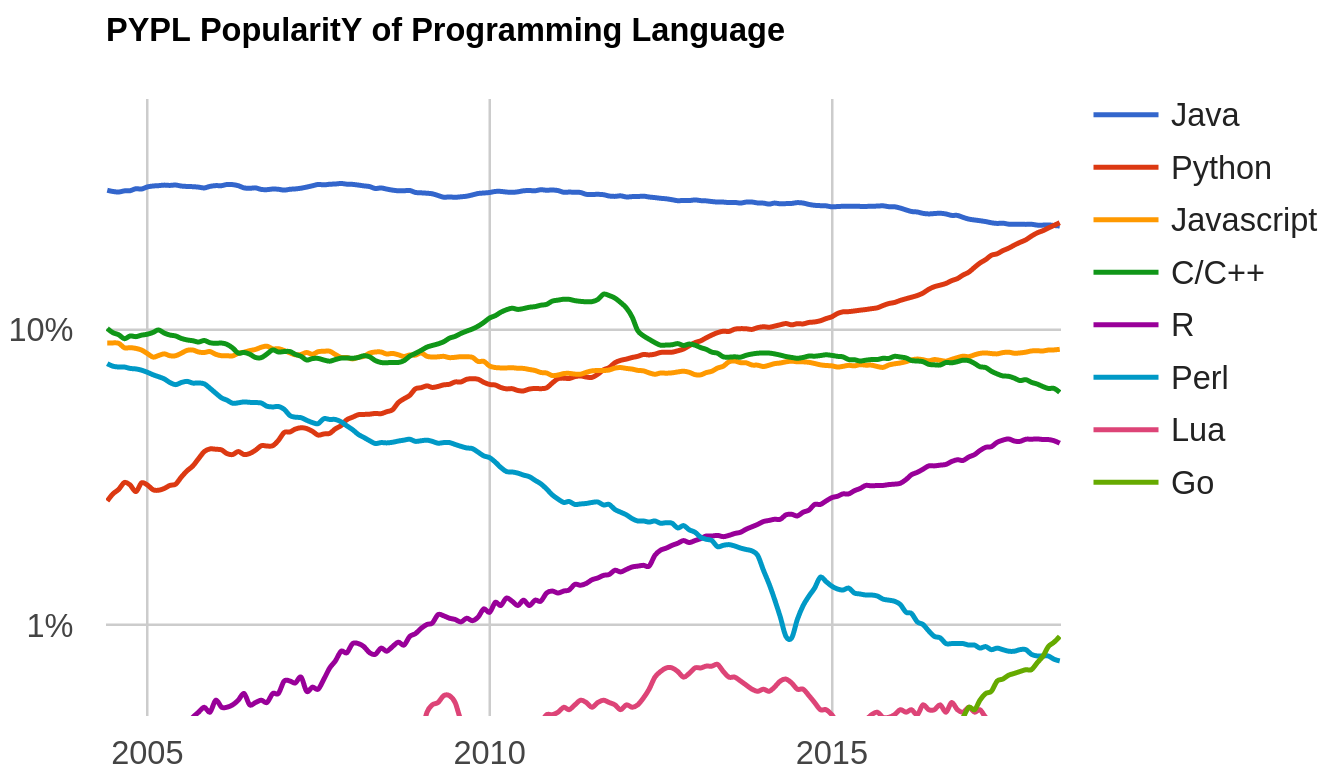
\includegraphics[width=0.8\linewidth]{pypl-popularity.png}
\end{center}
\textcolor{blue}{\scriptsize\url{http://pypl.github.io/PYPL.html}}
\end{frame}

\begin{frame}{Why we're here}
\vspace{0.5 cm}
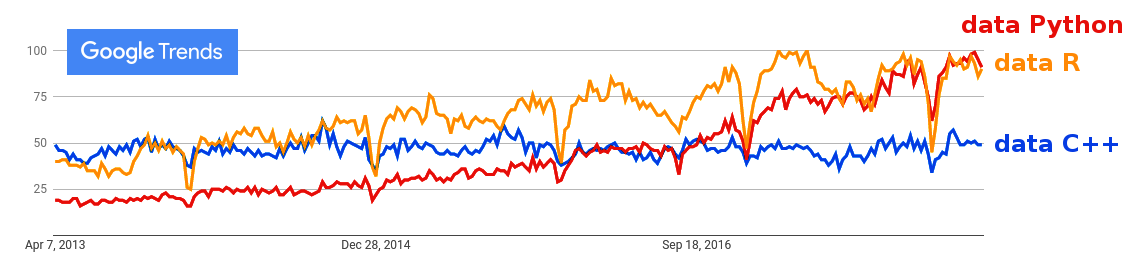
\includegraphics[width=\linewidth]{python-r-cpp-googletrends-data.png}

\vspace{1 cm}
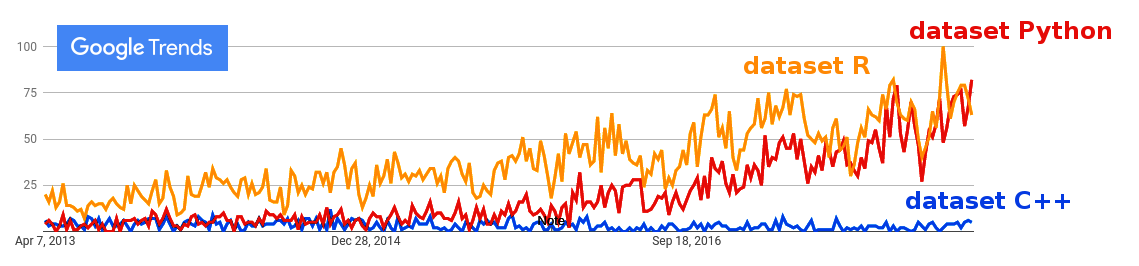
\includegraphics[width=\linewidth]{python-r-cpp-googletrends-dataset.png}
\end{frame}

\begin{frame}{Why we're here}
\vspace{0.5 cm}
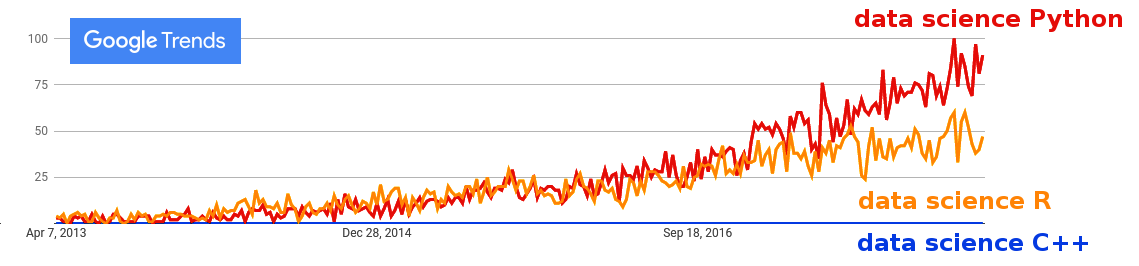
\includegraphics[width=\linewidth]{python-r-cpp-googletrends-datascience.png}

\vspace{1 cm}
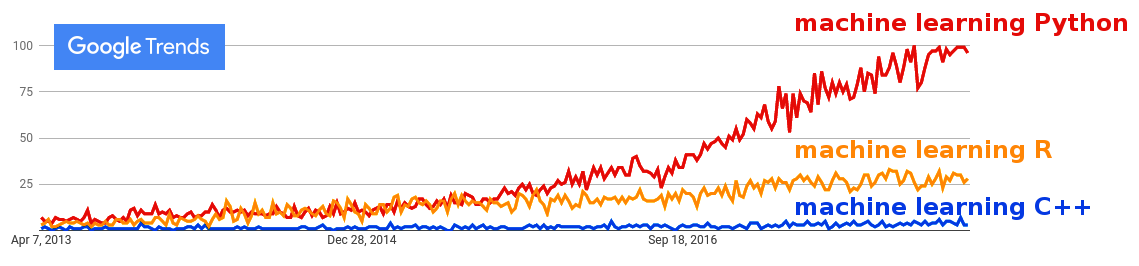
\includegraphics[width=\linewidth]{python-r-cpp-googletrends-machinelearning.png}
\end{frame}

\begin{frame}{Why we're here}
\large
\vspace{0.4 cm}
All of the machine learning libraries I could find either have a Python interface or are primarily/exclusively Python.

\vspace{0.6 cm}
\mbox{ } 
\includegraphics[height=0.8 cm]{sklearn-logo.png}
\hfill 
\includegraphics[height=0.8 cm]{pytorch-logo.png}
\hfill 
\includegraphics[height=0.8 cm]{keras-logo.png}
\hfill 
\includegraphics[height=1 cm]{tensorflow-logo.png}
\hfill 
\includegraphics[height=0.8 cm]{caffe2-logo.png}
\hfill 
\includegraphics[height=0.8 cm]{gluon-logo.png} \mbox{ }

\vspace{0.15 cm}
\mbox{ } 
\includegraphics[height=0.8 cm]{chainer-logo.png}
\hfill 
\includegraphics[height=0.8 cm]{cntk-logo.png}
\hfill 
\includegraphics[height=0.8 cm]{lasagne-logo.png}
\hfill 
\includegraphics[height=0.8 cm]{onnx-logo.png}
\hfill 
\includegraphics[height=0.8 cm]{cesium-logo.png}
\hfill 
\includegraphics[height=0.8 cm]{xgboost-logo.png} \mbox{ }
\end{frame}

\begin{frame}{Why we're here}
\vspace{0.25 cm}
\begin{center}
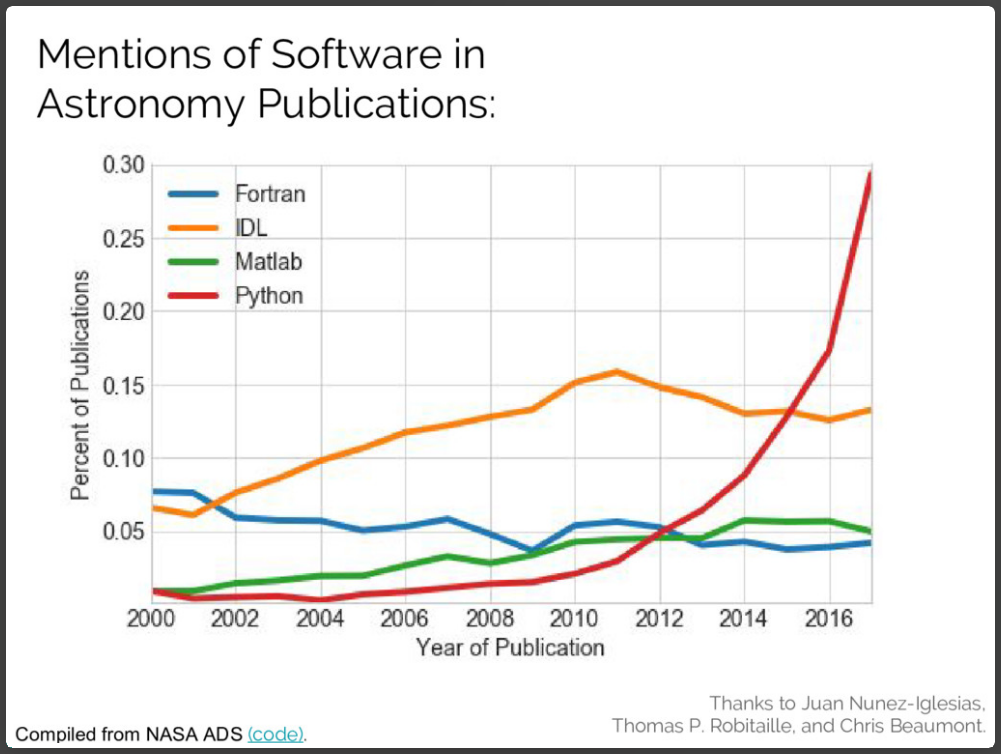
\includegraphics[width=0.7\linewidth]{mentions-of-programming-languages.png}
\end{center}
\end{frame}

\begin{frame}{Why we're here}
\large
\vspace{0.5 cm}
\textcolor{darkblue}{\huge Python in HEP?}

\vspace{0.5 cm}
\begin{itemize}\setlength{\itemsep}{0.5 cm}
\item<2-> Collaboration frameworks like Athena and CMSSW are configured or driven by Python.

\item<3-> Today, it is common for physicists to do their analyses in Python/PyROOT.

\vspace{0.1 cm}
\textcolor{gray}{\normalsize (Half Python, half C++? Anyway, a lot more than in LHC Run I.)}

\item<4-> Python is a bridge to machine learning and other statistical software written outside of HEP.
\end{itemize}
\end{frame}

\begin{frame}{}
\Large
\vspace{1 cm}
\textcolor{darkgray}{To be honest, Python isn't my favorite language.}

\large
\vspace{1 cm}
\uncover<2->{\textcolor{darkgray}{I wish the scientific and data analysis community had adopted something more functional and statically typed. In particular, I wish there wasn't a dichotomy between statements and expressions. And {\tt True == 1} is evil.}}

\large
\vspace{1 cm}
\uncover<3->{\textcolor{darkgray}{But a dash of consensus is well worth a smattering of language features\ldots}}
\end{frame}

\begin{frame}{Why Python?}
\large
\vspace{0.5 cm}
\begin{columns}[t]
\column{0.55\linewidth}
\underline{Did Python just arrive at the right time?}

\vspace{0.25 cm}
\begin{uncoverenv}<2->
\begin{itemize}
\item Ruby, Lua numerical stacks were not ready before Python already had a foothold.
\item Python was one of the first glue languages of the Linux/open source era.
\end{itemize}
\end{uncoverenv}

\column{0.5\linewidth}
\underline{Or is it a better language for the job?}

\vspace{0.25 cm}
\begin{uncoverenv}<3->
\begin{itemize}
\item Perl $\to$ Python
\item ``Tcl War''
\item R $\to$ Python
\item<4-> {\it An Empirical Investigation into Programming Language Syntax,} Andreas Stefik, Susanna Siebert.
\end{itemize}
\end{uncoverenv}
\end{columns}
\end{frame}

\begin{frame}{An Empirical Investigation into Programming Language Syntax}
\begin{columns}
\column{0.58\linewidth}
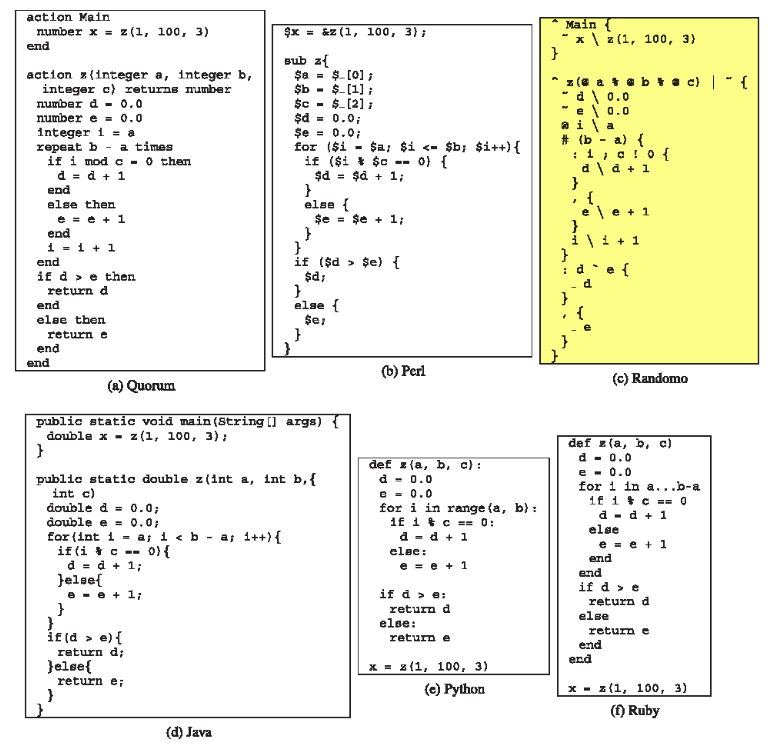
\includegraphics[width=\linewidth]{empirical-examples.png}

\column{0.42\linewidth}
\uncover<1>{\fcolorbox{black}{white}{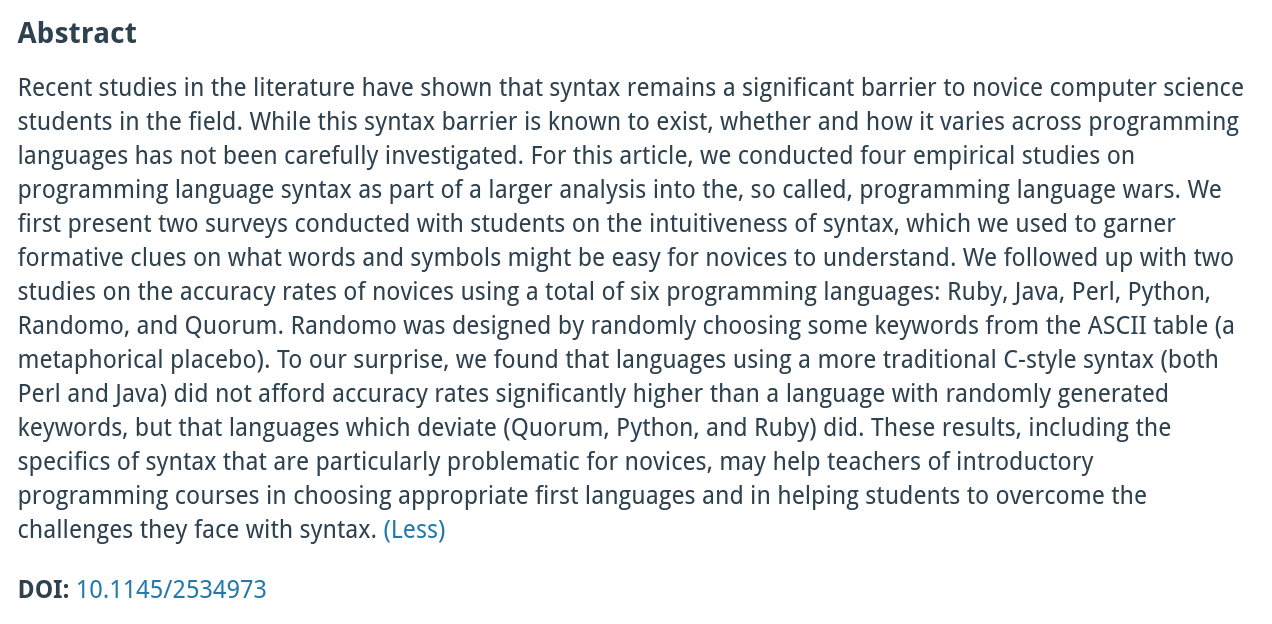
\includegraphics[width=\linewidth]{empirical-abstract.png}}}

\vspace{1 cm}
\mbox{\hspace{-1 cm}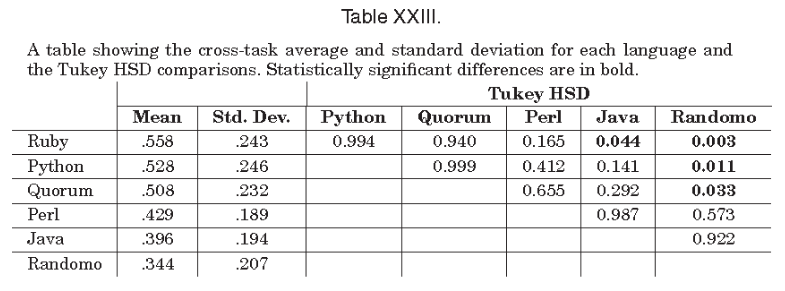
\includegraphics[width=1.25\linewidth]{empirical-table.png}}
\end{columns}

\vspace{-7.6 cm}
\begin{uncoverenv}<2->
\begin{center}
\fcolorbox{black}{white}{\begin{minipage}{0.85\linewidth}
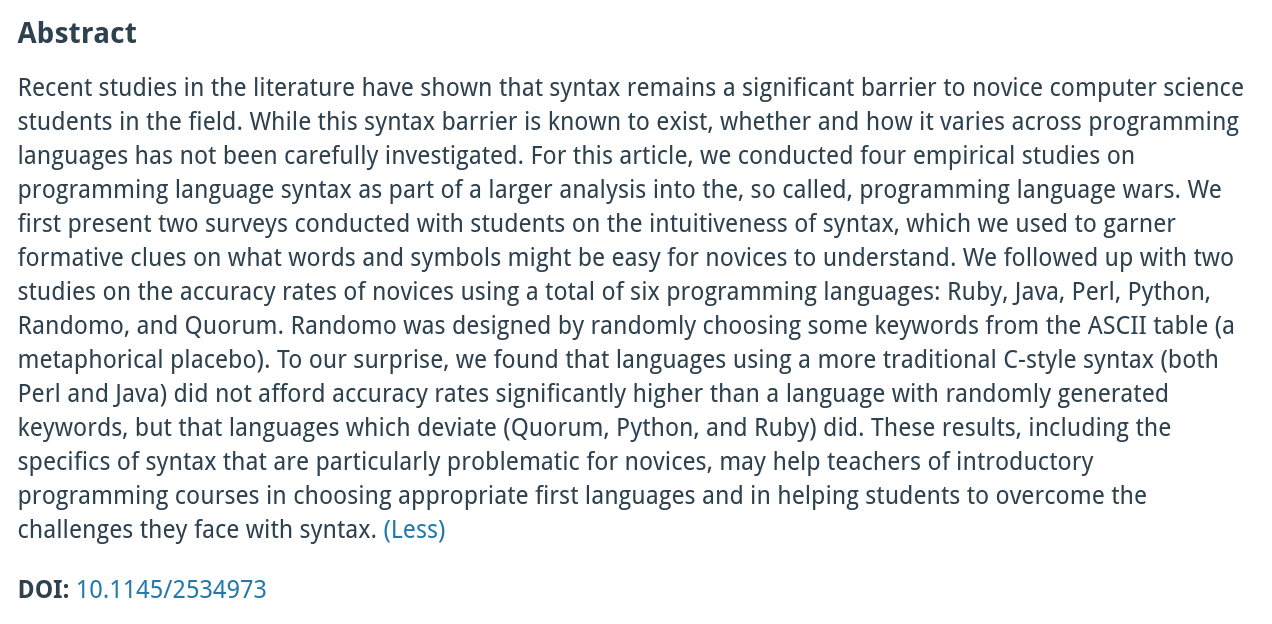
\includegraphics[width=\linewidth]{empirical-abstract.png}\end{minipage}}
\end{center}
\end{uncoverenv}
\end{frame}

\begin{frame}{My conclusion (debatable)}
\huge
\vspace{1 cm}
\begin{center}
Python was good enough and first.
\end{center}
\end{frame}

\begin{frame}{More significant: what has grown around Python}
\vspace{0.25 cm}
\begin{columns}[b]
\column{0.75\linewidth}
\only<1>{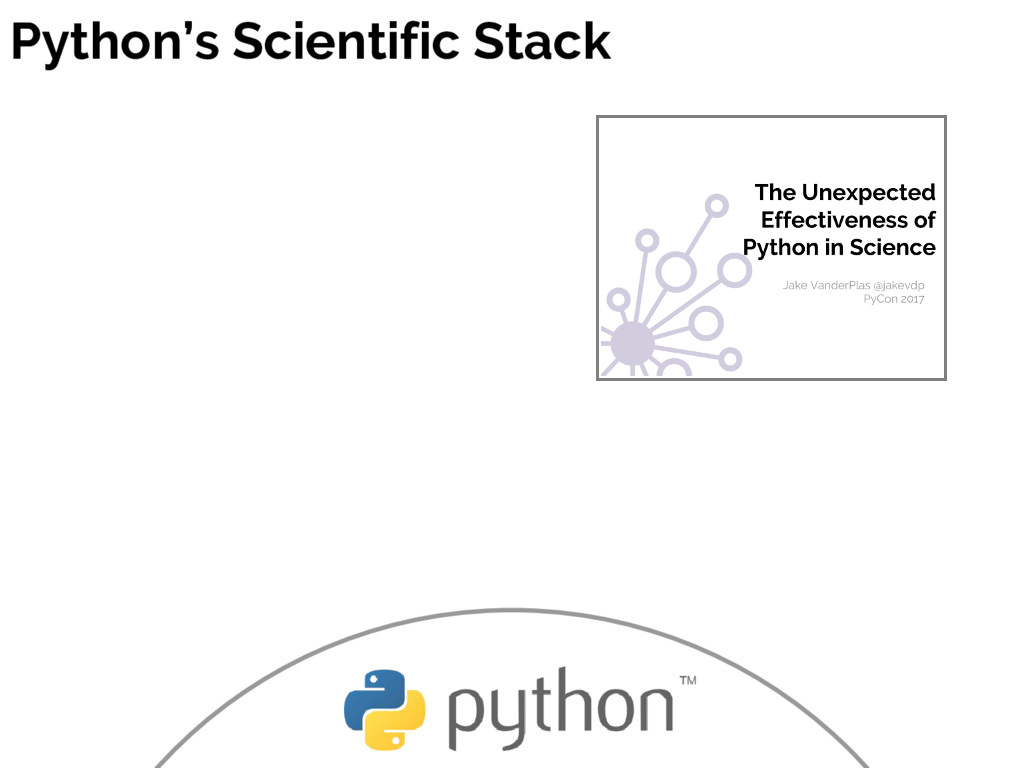
\includegraphics[height=7.8 cm]{shells-1.png}}
\only<2>{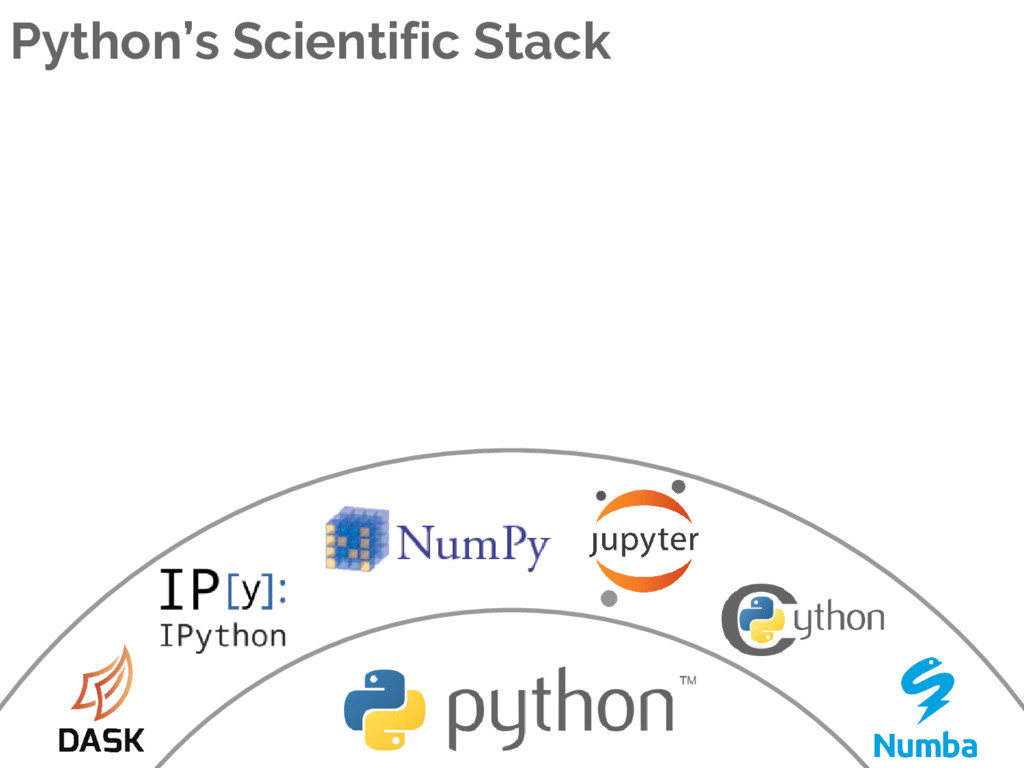
\includegraphics[height=7.8 cm]{shells-2.png}}
\only<3>{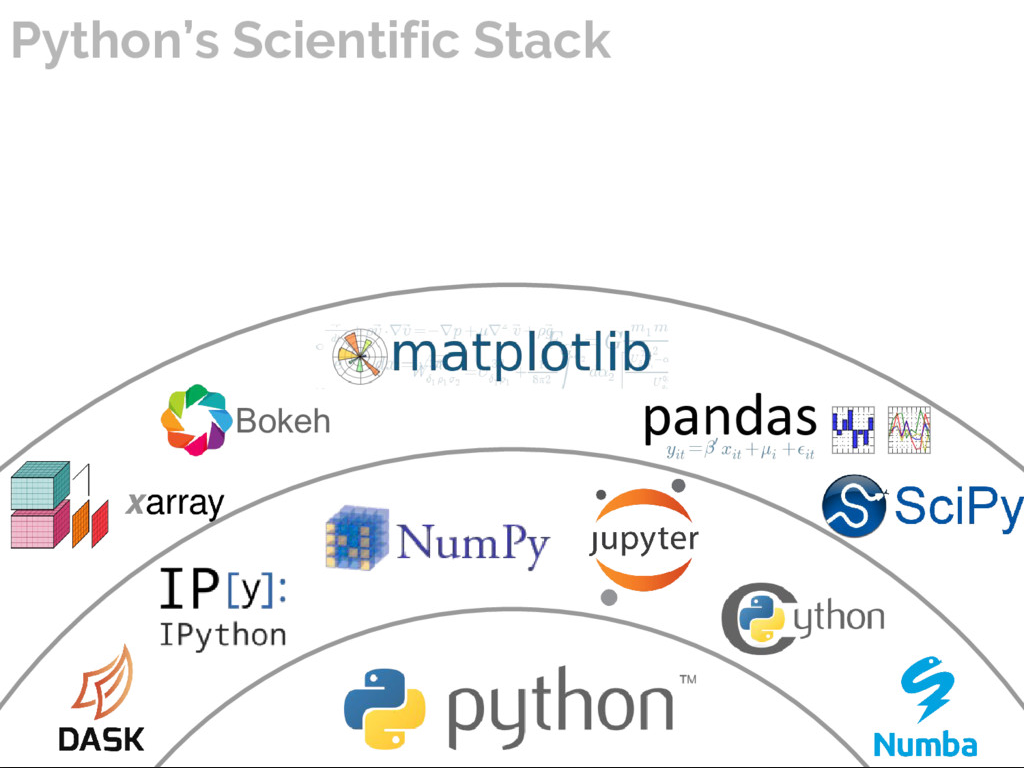
\includegraphics[height=7.8 cm]{shells-3.png}}
\only<4>{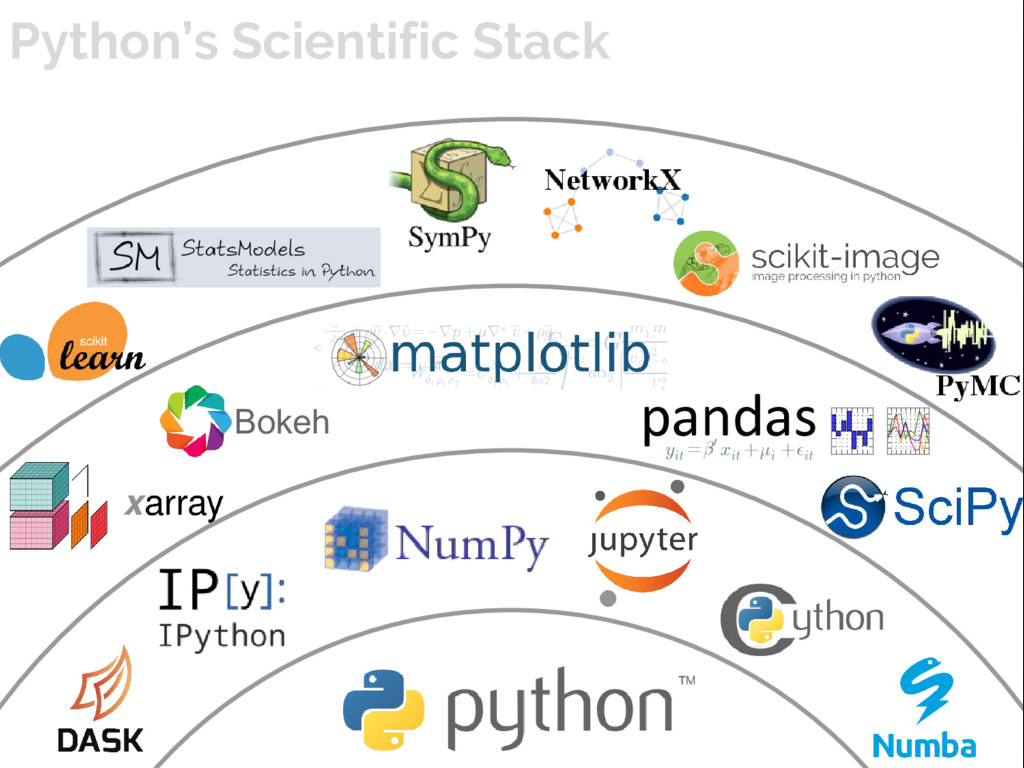
\includegraphics[height=7.8 cm]{shells-4.png}}
\only<5>{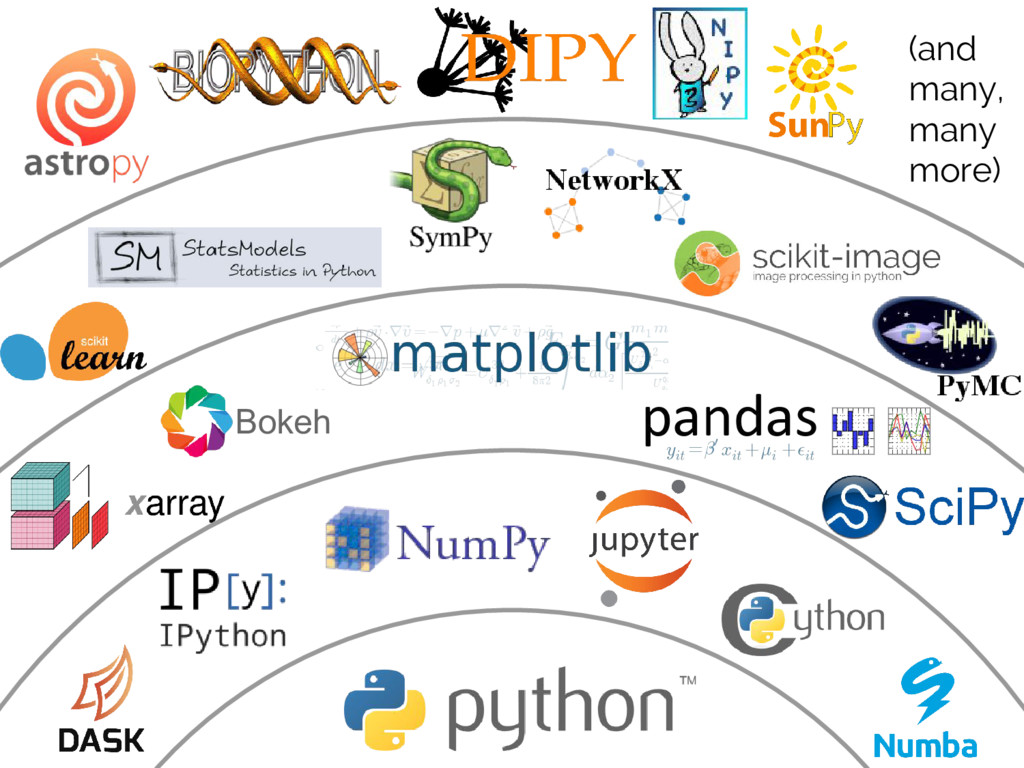
\includegraphics[height=7.8 cm]{shells-5.png}}

\column{0.25\linewidth}
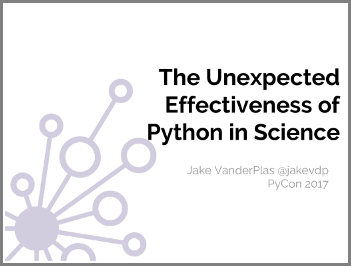
\includegraphics[width=\linewidth]{unreasonable-effectiveness.png}
\vspace{5.3 cm}
\end{columns}
\end{frame}

\begin{frame}{The key to ecosystem development was a good array library}
\large
\vspace{0.3 cm}

\renewcommand{\arraystretch}{1.15}
\mbox{\hspace{-0.5 cm}\begin{tabular}{c p{0.95\linewidth}}
1994 & \textcolor{darkorange}{\bf Python} 1.0 released. \\
1995 & First array package: \textcolor{darkorange}{\bf Numeric} \textcolor{gray}{(a.k.a.\ Numerical, Numerical Python, NumPy).} \\
2001 & Diverse scientific codebases merged into \textcolor{darkorange}{\bf SciPy}. \\
2003 & \textcolor{darkorange}{\bf Matplotlib} \\
2003 & Numeric was limited; \textcolor{darkorange}{\bf numarray} appeared as a competitor with more \mbox{features} \textcolor{gray}{(memory-mapped files, alignment, record arrays)}. \\
2005 & Two packages were incompatible; could not integrate numarray-based code into SciPy. Travis Oliphant merged the codebases as \textcolor{darkorange}{\bf Numpy}. \\
2008 & \textcolor{darkorange}{\bf Pandas} \\
2010 & \textcolor{darkorange}{\bf Scikit-Learn} \\
2011 & \textcolor{darkorange}{\bf AstroPy} \\
2012 & \textcolor{darkorange}{\bf Anaconda} \\
2014 & \textcolor{darkorange}{\bf Jupyter} \\
2015 & \textcolor{darkorange}{\bf Keras} \\
\end{tabular}}
\end{frame}

\begin{frame}[fragile]{Numpy is high-level, array-at-a-time math}
\vspace{0.5 cm}
\hfill 
\includegraphics[height=1.5 cm]{numpy-logo.png}

\scriptsize
\vspace{-1.5 cm}
\begin{minted}{python}
>>> import numpy
>>> a = numpy.arange(12)
>>> a
array([ 0,  1,  2,  3,  4,  5,  6,  7,  8,  9, 10, 11])
>>> a.shape = (3, 4)
>>> a
array([[ 0,  1,  2,  3],
       [ 4,  5,  6,  7],
       [ 8,  9, 10, 11]])
>>> a.sum(axis=0)
array([12, 15, 18, 21])
>>> a.min(axis=1)
array([0, 4, 8])
>>> a**2
array([[  0,   1,   4,   9],
       [ 16,  25,  36,  49],
       [ 64,  81, 100, 121]])
>>> numpy.sqrt(a)
array([[0.        , 1.        , 1.41421356, 1.73205081],
       [2.        , 2.23606798, 2.44948974, 2.64575131],
       [2.82842712, 3.        , 3.16227766, 3.31662479]])
\end{minted}
\end{frame}

\begin{frame}[fragile]{Numpy is also a low-level way to poke raw bytes}
\vspace{0.5 cm}
\hfill 
\includegraphics[height=1.5 cm]{numpy-logo.png}

\scriptsize
\vspace{-1.5 cm}
\begin{minted}{python}
>>> import numpy
>>> hello = b"Hello, world!"

>>> # Python strings are immutable
>>> hello[4:8] = "????"
Traceback (most recent call last):
  File "<stdin>", line 1, in <module>
TypeError: 'bytes' object does not support item assignment

>>> # any buffer may be cast as an array
>>> a = numpy.frombuffer(hello, dtype=numpy.uint8)
>>> a
array([ 72, 101, 108, 108, 111,  44,  32, 119, 111, 114, 108, 100,  33],
      dtype=uint8)

>>> # and changed (with possibly disastrous consequences)
>>> a.flags.writeable = True
>>> a[4:8] = [69, 86, 73, 76]
>>> hello
b'HellEVILorld!'
\end{minted}
\end{frame}

\begin{frame}[fragile]{Numpy is also a low-level way to poke raw bytes}
\vspace{0.5 cm}
\hfill 
\includegraphics[height=1.5 cm]{numpy-logo.png}

\scriptsize
\vspace{-1.5 cm}
\begin{minted}{python}
>>> # any *pointer* may be cast as an array
>>> ptr = ctypes.cast(id(hello), ctypes.POINTER(ctypes.c_uint8))
>>> ptr.__array_interface__ = {
...     "version": 3,
...     "typestr": numpy.ctypeslib._dtype(type(ptr.contents)).str,
...     "data": (ctypes.addressof(ptr.contents), False),
...     "shape": (100,)    # how much memory do you want to poke?
... }
... 
>>> b = numpy.array(ptr, copy=False)
>>> b
array([  2,   0,   0,   0,   0,   0,   0,   0, 224, 136, 151,   0,   0,
         0,   0,   0,  13,   0,   0,   0,   0,   0,   0,   0,  47,  49,
       110, 120,  37, 235,  98,  94,  72, 101, 108, 108,  69,  86,  73,
        76, 111, 114, 108, 100,  33,   0,   0,   0,   1,   0,   0,   0,
         0,   0,   0,   0, 224, 136, 151,   0,   0,   0,   0,   0,  12,
         0,   0,   0,   0,   0,   0,   0, 255, 255, 255, 255, 255, 255,
       255, 255,   0,   1,  18,   1,   3,   1,  22,   1,  13,   1,   5,
         1,   0, 105,   0,   0,   1,   0,   0,   0], dtype=uint8)
>>> "".join(map(chr, b[32:45]))
'HellEVILorld!'
\end{minted}
\end{frame}


\end{document}



%% https://speakerdeck.com/jakevdp/the-unexpected-effectiveness-of-python-in-science
